\documentclass{article}

\usepackage[english]{babel}
\usepackage{amsfonts, amsmath, amssymb, MnSymbol, graphicx, hyperref, amsthm, algorithmicx, algpseudocode}
\usepackage[Algorithm,ruled]{algorithm}

%~~~~~~~~~~~~~~~~~~~~~~~~~~~~~~~~
% Math Shortcuts
\newcommand{\mbrace}[1]{\ensuremath{\left\{#1\right\}}}
\newcommand{\rpm}{\ensuremath{\raisebox{0.5ex}{$\scriptstyle\pm$}}}
\newcommand{\bfm}{\ensuremath{\mathbf{\mu}}}
\newcommand{\bfs}{\ensuremath{\mathbf{\sigma}}}
\newcommand{\mbf}[1]{\ensuremath{\mathbf{#1}}}
\newcommand{\mc}[1]{\ensuremath{\mathcal{#1}}}
\newcommand{\mkpartial}[2]{\ensuremath{\frac{\partial #1}{\partial #2}}}

%~~~~~~~~~~~~~~~~~~~~~~~~~~~~~~~~
% algpseudocode helpers
\newcommand{\algtab}{\hspace{\algorithmicindent}}
\newcommand{\algtitle}[1]{\smallskip\hrule\smallskip{\bf #1}\smallskip\hrule}

\newenvironment{algo}[1]
{\noindent\ignorespaces\algtitle{#1}\begin{algorithmic}[1]}
{\end{algorithmic}\hrule\smallskip\ignorespacesafterend}

%~~~~~~~~~~~~~~~~~~~~~~~~~~~~~~~~
% Formatting Shortcuts
\newcommand{\imgwidth}{.8\textwidth}
\newcommand{\result}[1]{\subsubsection*{#1}}
\newcommand{\fakesection}[1]{\noindent{\bf #1}\par}

%%%%%%%%%%%%%%%%%%%%%%%%%%%%%%%%%%%%%%%%%%%%%%%%%%%%%%%%%%%%%%%%%%%%%%%%%%%%%%%%%%%

\title{CAP5638 Project 2\\\smallskip
\large Classification Using Linear Discriminant Functions and Boosting Algorithms}
\author{Suhib Sam Kiswani}
\date{December 2, 2015}

%%%%%%%%%%%%%%%%%%%%%%%%%%%%%%%%%%%%%%%%%%%%%%%%%%%%%%%%%%%%%%%%%%%%%%%%%%%%%%%%%%%

\begin{document}
\maketitle

The algorithms were implemented in Python 3.5, with a dependence on the \textit{scipy}~\cite{sp} library.

%%%%%%%%%%%%%%%%%%%%%%%%%%%%%%%%%%%%%%%%%%%%%%%%%%%%%%%%%%%%%%%%%%%%%%%%%%%%%%%%%%%

\section{Basic Two-Class Classification Using Perceptron Algorithms}
Abstractly, the problem is as follows:
Given $n$ labeled training samples, $D=\{( x_1, L_1), (x_2, L_2), ..., (x_n, L_n)\}$, where $L_i = \rpm1$, implement Algorithm 4 (Fixed-Increment Single-Sample Perceptron Algorithm) and Algorithm 8 (Batch Relaxation with Margin) of Chapter 5 in the textbook \cite{duda}.

\bigskip

The algorithms are:
\begin{algo}{Algorithm 5.4 (Fixed-Increment Single-Sample Perceptron)}
\State {\bf initialize} $a,k = 0$
\State {\bf do} ~$k \gets (k+1)\mod n$
\State \algtab {\bf if} $\mbf{y}_k$ is misclassified by {\bf a} {\bf then} $\mbf{a} \gets \mbf{a} + \mbf{y}_k$
\State {\bf until} all patterns properly classified
\State {\bf return} $a$
\end{algo}
\bigskip
\begin{algo}{Algorithm 5.8 (Batch Relaxation with Margin)}
\State {\bf initialize} $a,\eta(\cdot),b,k \gets 0$
\State {\bf do} ~$k \gets (k+1)\mod n$
\State\algtab $\mc{Y}_k = \{\}$
\State\algtab $j = 0$
\State\algtab {\bf do} ~$j \gets j + 1$
\State\algtab\algtab {\bf if} $\mbf{a}^t\mbf{y}^j \leq b$ {\bf then} Append $\mbf{y}^j$ to $\mc{Y}_k$
\State\algtab {\bf until} ~$j = n$
\State\algtab $\mbf{a} \gets \mbf{a} + \eta(k)\sum_{y\in\mc{Y}}\frac{b-\mbf{a}^t\mbf{y}}{||\mbf{y}||^2}\mbf{y}$
\State {\bf until} $\mc{Y}_k = \{\}$
\State {\bf return} $a$
\end{algo}

%~~~~~~~~~~~~~~~~~~~~~~~~~~~~~~~~
\subsection*{Results}
Long training times proved problematic, due to the fact that it took greater than 100000 iterations to reach convergence using the fixed relaxation rule for the UCI wine data set. As such, the most significant result here is that the higher dimensional USPS handwritten digits data set converges much more rapidly than the UCI wine data set -- by several orders of magnitude. Futhermore, for the fixed-increment rule, accuracy is much greater when testing on the handwritten digits data set. The batch relaxation rule performed well for both data sets, though higher on average for the UCI wine data set.

This most likely has to do with the fact that the handwritten digits data set has a great deal more training samples than the wine data set. With more training samples to update the hyperplane, the classifier can converge to a solution much more rapidly. 

As for the long training times for the wine data set, the updated weights $\mbf{a}(k)$ would oscillate between values for a long time before settling on a steady solution. To prevent this behaviour, several early termination heuristics were used. The heuristics were:
\begin{enumerate}
\item Always terminate after 100,000 iterations, and using the value of $\mbf{a}$ that minimizes $J_p(\mbf{a})$ for Algorithm 5.4 and $J_r(\mbf{a})$ for Algorithm 5.8.
\item Terminate if, after 50,000 iterations, $||\mbf{a}(k+1) - \mbf{a}(k)|| \approx 0$, and $J_p(\mbf{a}) \approx 0$ for Algorithm 5.4 and $J_r(\mbf{a})\approx 0$ for Algorithm 5.8.
\end{enumerate}

Most likely, the necessity for early termination is due to the fact that the mean and standard deviation of the training samples was not normalized (however, the perceptron was trained using normalized augmented features, e.g. for training label $\omega_1$, $y^T_i = [1, \mbf{x_i}]$ if $x_i$ belongs to $\omega_1$, and $y^T_i = [-1, -\mbf{x_i}]$ if $x_i$ is not a sample for $\omega_1$.

It's very likely that these early-termination heuristics had a detrimental effect on the classification accuracy, since in these cases, the there was no guarantee that $\mbf{a}^T\mbf{y} \geq 0$ for all augmented $\mbf{y}$.

\result{UCI Wine Data Set}
\fakesection{Algorithm 5.4 (Fixed-Increment Single-Sample Perceptron)}
\begin{center}
\begin{tabular}{|c|c|c|c|}
\hline\multicolumn{4}{|c|}{{\bf Training Statistics}}\\
\hline{\bf Class} & {\bf Correct (of 89) (\%)} & {\bf Iterations} & {\bf Runtime(s)}\\\hline
$\omega_1$ & 60 (67.42\%) & 100001 & 63.151 \\
$\omega_2$ & 56 (62.92\%) & 100001 & 63.050 \\
$\omega_3$ & 85 (95.51\%) & 84710 & 53.850\\
\hline
{\bf Total} & ~ & 284710 & 180.051\\
\hline
\end{tabular}
\end{center}

The corresponding weights after training were:
\begin{center}
\begin{tabular}{ ccc }
$\mbf{a}_{\omega_1} = \left[\begin{matrix}
-2.\\-23.54\\-1.28\\-3.54\\-36.8\\-136.\\-2.7\\0.36\\-1.34\\2.3\\-2.86\\-2.88\\-0.42\\-490.
\end{matrix}\right]$ &
$\mbf{a}_{\omega_2} = \left[\begin{matrix}
9484.0\\56298.47\\-26970.62\\9950.26\\-10456.6\\-3765.\\55712.08\\-1502.68\\36611.34\\-40821.68\\-109006.33\\65677.49\\44053.19\\-430.0
\end{matrix}\right]$ &
$\mbf{a}_{\omega_3} = \left[\begin{matrix}
451.0\\-1399.63\\-10081.3\\-16667.88\\28250.3\\2665.0\\-71066.41\\-107364.33\\-12267.75\\-24570.91\\94303.98\\-52048.4\\-132265.0\\-958.0
\end{matrix}\right]$
\end{tabular}
\end{center}

\bigskip

\fakesection{Algorithm 5.8 (Batch Relaxation with Margin)}

\begin{center}
\begin{tabular}{|c|c|c|c|}
\hline\multicolumn{4}{|c|}{{\bf Training Statistics}}\\
\hline{\bf Class} & {\bf Correct (of 89) (\%)} & {\bf Iterations} & {\bf Runtime(s)}\\\hline
$\omega_1$ & 87 (97.75\%) & 22864 & 27.498 \\
$\omega_2$ & 85 (95.51\%) & 52918 & 62.130 \\
$\omega_3$ & 83 (93.26\%) & 35600 & 127.227\\
\hline
{\bf Total} & ~ & 111,382 & 216.855\\
\hline
\end{tabular}
\end{center}

The corresponding weights after training were:
\begin{center}
\begin{tabular}{ ccc }
$\mbf{a}_{\omega_1} = \left[\begin{matrix}
0.796\\-0.31 \\ 0.768 \\ 0.183 \\ -0.362 \\ -0.063 \\  0.74 \\ 0.153 \\ 0.867 \\  0.601 \\ 0.128 \\ 0.216 \\ 0.583 \\ 0.01
\end{matrix}\right]$ &
$\mbf{a}_{\omega_2} = \left[\begin{matrix}
261.354 \\ 869.172 \\ -1800.878 \\ -101.749 \\ 1335.277\\6.557\\1335.119\\1928.754\\99.223\\921.129\\-6428.793\\895.385\\2459.442\\-33.943
\end{matrix}\right]$ &
$\mbf{a}_{\omega_1} = \left[\begin{matrix}
0.855\\-0.161\\0.587\\0.188\\-0.108\\-0.017\\0.295\\-0.334\\0.758\\-0.18\\0.882\\-0.084\\0.086\\-0.003
\end{matrix}\right]$
\end{tabular}
\end{center}

\result{USPS Handwritten Digits Data Set}
\fakesection{Algorithm 5.4 (Fixed-Increment Single-Sample Perceptron)}

\begin{center}
\begin{tabular}{|c|c|c|c|}
\hline\multicolumn{4}{|c|}{{\bf Training Statistics}}\\
\hline{\bf Class} & {\bf Correct (of 2007) (\%)} & {\bf Iterations} & {\bf Runtime(s)}\\\hline
$\omega_0$ & 1928 (96.06\%) &17 trials & 0.031\\
$\omega_1$ & 1982 (98.75\%) & 9 trials & 0.018\\
$\omega_2$ & 1873 (93.32\%) & 14 trials & 0.026\\
$\omega_3$ & 1896 (94.47\%) & 14 trials & 0.033\\
$\omega_4$ & 1897 (94.52\%) & 23 trials & 0.040\\
$\omega_5$ & 1905 (94.92\%) & 22 trials & 0.042\\
$\omega_6$ & 1960 (97.66\%) & 25 trials & 0.047\\
$\omega_7$ & 1926 (95.96\% & 25 trials & 0.045\\
$\omega_8$ & 1881 (93.72\%) & 20 trials & 0.037\\
$\omega_9$ & 1919 (95.62\%) & 41 trials & 0.073\\
\hline
{\bf Total} & ~ & 210 & 0.392\\
\hline
\end{tabular}
\end{center}

The weights are too large to display in the report, however they can be displayed by invoking the following command using the included run.py script:
\begin{center}
python3 run.py fixed bin/digits\_train.txt bin/digits\_test.txt
\end{center}

\bigskip

\fakesection{Algorithm 5.8 (Batch Relaxation with Margin)}

\begin{center}
\begin{tabular}{|c|c|c|c|}
\hline\multicolumn{4}{|c|}{{\bf Training Statistics}}\\
\hline{\bf Class} & {\bf Correct (of 2007) (\%)} & {\bf Iterations} & {\bf Runtime(s)}\\\hline
$\omega_0$ & 1837 (91.53\%) & 717 & 1.297 \\
$\omega_1$ & 1917 (95.52\%) & 742 & 1.277 \\
$\omega_2$ & 1850 (92.18\%) & 606 & 1.084 \\
$\omega_3$ & 1894 (94.37\%) & 434 & 0.744 \\
$\omega_4$ & 1843 (91.83\%) & 597 & 1.130 \\
$\omega_5$ & 1900 (94.67\%) & 825 & 1.571 \\
$\omega_6$ & 1891 (94.22\%) & 831 & 1.612 \\
$\omega_7$ & 1904 (94.87\%) & 1358 & 2.581 \\
$\omega_8$ & 1863 (92.83\%) & 934 & 1.907 \\
$\omega_9$ & 1898 (94.57\%) & 1649 & 3.331 \\
\hline
{\bf Total} & ~ & 18797 & 16.535\\
\hline
\end{tabular}
\end{center}

The weights are too large to display in the report, however they can be displayed by invoking the following command using the included run.py script:
\begin{center}
python3 run.py relax bin/digits\_train.txt bin/digits\_test.txt
\end{center}

%%%%%%%%%%%%%%%%%%%%%%%%%%%%%%%%%%%%%%%%%%%%%%%%%%%%%%%%%%%%%%%%%%%%%%%%%%%%%%%%%%%
\section{Multi-Class Classification}
%Use the basic two-class perceptron algorithms to solve multi-class classification problems by using the one-against-the-rest and one-against-the-other methods. Note that you need to handle ambiguous cases properly.
For this classification method, both the fixed-increment and batch relaxation training rules from the previous section were used for testing.

For one-against-the-rest classification, a sample was classified as $\omega_i$ if $\mbf{a}^T_i \mbf{x} \geq \mbf{a}^T_j \mbf{x}$ for all $i \neq j$.


For one-against-other classification...
{\huge TODO}


%~~~~~~~~~~~~~~~~~~~~~~~~~~~~~~~~
\subsection*{Results}
%For each dataset, now train a classifier to classify all the classes using the one-against-the-rest and the one-against-the-other methods based on the two two-class algorithms, resulting in four different classifiers on each dataset and then classify the test set. Document classification accuracy, iterations in training, and classification time for test, and compare the one-against-the- rest and the one-against-the-other methods.
\emph{(Note: The runtime statistics for training are tabulated in the previous section)}

\result{UCI Wine Data Set}

\fakesection{One-Against-the-Rest}
Using the fixed increment rule (Algorithm 5.4 above), the one-against-the-rest classifier correctly classified 68 testing samples out of 89 (76.40\% accuracy). There were 111382 iterations during training (taking $\approx 216.855$ seconds). 
\begin{center}
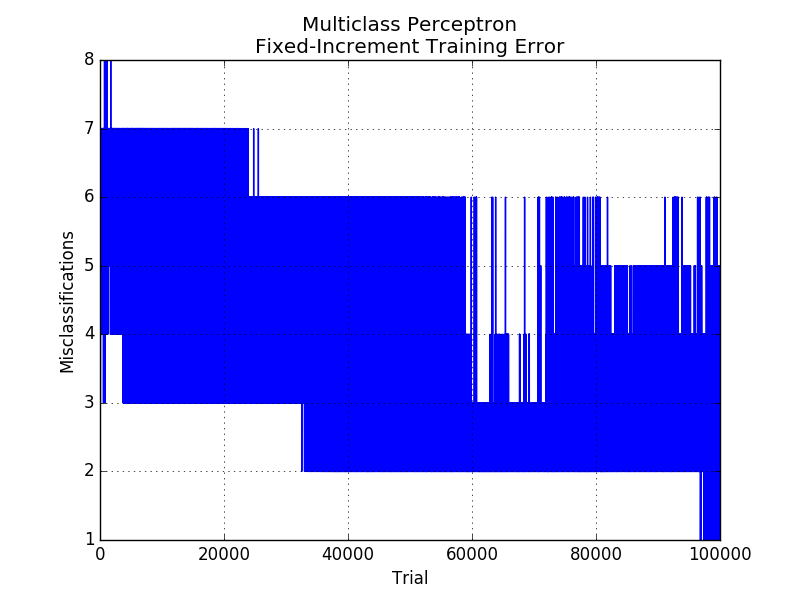
\includegraphics[width=\imgwidth]{mc_ovr_wine_fixed}
\end{center}

\bigskip

Using the batch relaxation rule (Algorithm 5.8), the one-against-the-rest classifier correctly classified 85 testing samples out of 89 (95.51\% accuracy). There were 300000 iterations during training (taking $\approx 398.827$ seconds). 
\begin{center}
\includegraphics[width=\imgwidth]{mc_ovr_wine_batch}
\end{center}

\bigskip
\fakesection{One-Against-the-Other}

{\Huge TODO}

\bigskip
\result{USPS Handwritten Digits Data Set}
\fakesection{One-Against-the-Rest}
{\large Completed training after 27 trials. Total training time: 2.923
1617 correct out of 2007 (80.57 accuracy)}

Using the fixed increment rule (Algorithm 5.4 above), the one-against-the-rest classifier correctly classified 1608 samples out of 2007 (80.12\% accuracy). Training occured over 177 iterations ($\approx 0.571$ seconds).
\begin{center}
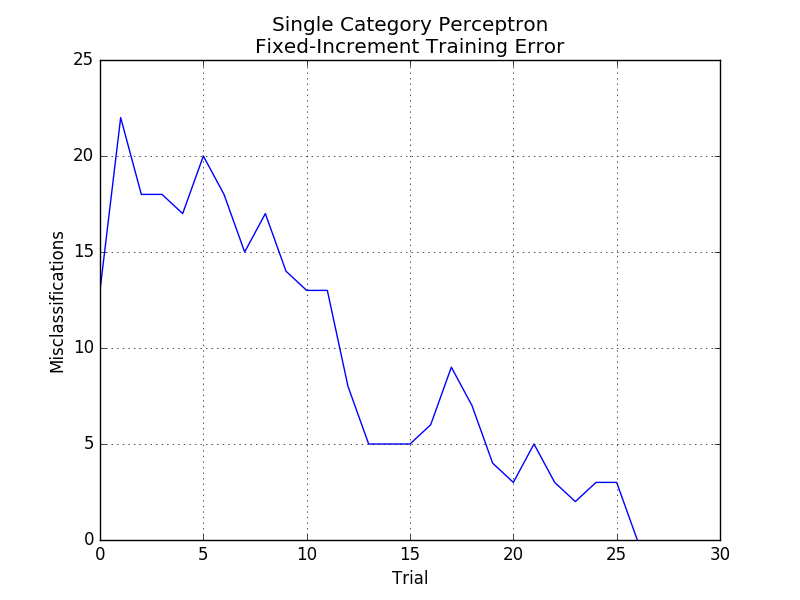
\includegraphics[width=\imgwidth]{mc_ovr_digits_fixed}
\end{center}

Using the batch relaxation rule (Algorithm 5.8), the one-against-the-rest classifier correctly classified 1626 testing samples out of 2007 (81.02\% accuracy). Training occured over 142 training trials ($\approx 23.032$ seconds).
\begin{center}
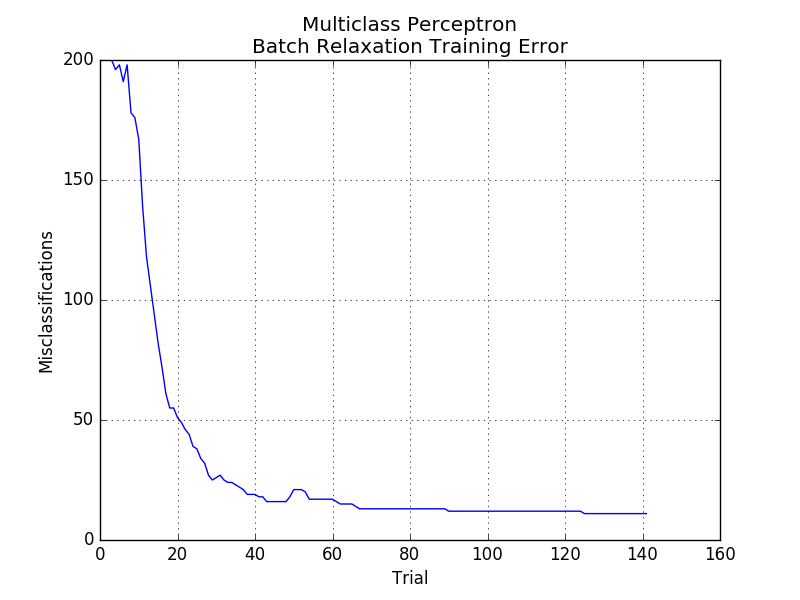
\includegraphics[width=\imgwidth]{mc_ovr_digits_batch}
\end{center}


\fakesection{One-Against-the-Other}


%%%%%%%%%%%%%%%%%%%%%%%%%%%%%%%%%%%%%%%%%%%%%%%%%%%%%%%%%%%%%%%%%%%%%%%%%%%%%%%%%%%

\section{Adaboost to Create Strong Classifers}
Implement Algorithm 1 (AdaBoost) in Chapter 9 of the textbook to create a strong classifier using the above linear discriminant functions.

\begin{figure}[H]
\begin{algo}{Algorithm 9.1 (AdaBoost)}
\newcommand{\mbx}{\mbf{x}}
\State {\bf initialize} $\mc{D} = \mbrace{\mbx^1, y_1, ..., \mbx^n, y_n}, k_{max}, W_1(i) = 1/n, i = 1...n$
\State $k = 0$
\State {\bf do} ~$k \gets k+1$
\State\algtab train weak learner $C_k$ using \mc{D} sampled according to $W_k(i)$
\State\algtab $E_k \gets$ training error of $C_k$ measured on \mc{D} using $W_k(i)$
\State\algtab $\alpha_k \gets 0.5 \ln\left[ (1-E_k) / E_k \right]$
\State\algtab $W_{k+1}(i) = \frac{W_k(i)}{Z_k} \times \begin{cases}
e^{-\alpha_k} & \text{ if } h_x(\mbx^i) = y_i \text{ (correct classification)}\\
e^{\alpha_k} & \text{ if } h_k(\mbx^i) \neq y_i \text{ (incorrect classification)}
\end{cases}$
\State {\bf until} $k = k_{max}$
\State {\bf return} $C_k$ and $\alpha_k$ for $k = 1$ to $k_{max}$ (ensemble of classifiers with weights)
\end{algo}
\end{figure}

%~~~~~~~~~~~~~~~~~~~~~~~~~~~~~~~~
\subsection*{Results}
Boost Algorithm 8 to create a strong classifier for class 1 vs. class 2, class 1 vs. class 3, and class 2 vs. class 3 on the two datasets. Then classify the corresponding test samples from the relevant classes in test sets (in other words, for example, for the class 1 vs. class 2 classifier, you only need to classify test samples from classes 1 and 2); then document classification accuracy and show and analyze the improvement.

\bigskip

\fakesection{UCI Wine Data Set}
\bigskip
\fakesection{USPS Handwritten Digits Data Set}


%%%%%%%%%%%%%%%%%%%%%%%%%%%%%%%%%%%%%%%%%%%%%%%%%%%%%%%%%%%%%%%%%%%%%%%%%%%%%%%%%%%

\section{Extra Credit}
\subsection{Support vector machines}
By using an available quadratic programming optimizer or an SVM library, implement a training and classification algorithm for support vector machines. Then use your algorithm on the USPS dataset. Document the classification accuracy and compare the results with that from the two basic algorithms.

\subsubsection*{Results}
{\large TODO}

%%%%%%%%%%%%%%%%%%%%%%%%%%%%%%%%%%%%%%%%%%%%%%%%%%%%%%%%%%%%%%%%%%%%%%%%%%%%%%%%%%%

\subsection{Kernel method for linear discriminant functions}
Given a kernel function, derive the kernel-version of Algorithm 4 and implement the algorithm, and then apply it on the given wine and USPS datasets. Document the classification accuracy and compare the results with that from the two basic algorithms without kernels. Use the polynomial function of degree three as the kernel function; optionally, you can use other commonly used kernel functions.

\subsubsection*{Results}
{\large TODO}


%%%%%%%%%%%%%%%%%%%%%%%%%%%%%%%%%%%%%%%%%%%%%%%%%%%%%%%%%%%%%%%%%%%%%%%%%%%%%%%%%%%

\subsection{Multiple-class linear machines and multiple-class boosting}
Use the Kesler’s construction to train a linear machine for multi-class classification and then use the SAMME algorithm to boost its performance on the training set. Apply the algorithm on both datasets and classify the corresponding test samples in the test sets. Document the classification accuracy and compare the results with that from the one-against-the-rest and one-against-the- other algorithms.

\subsubsection{Results}
{\large TODO}

%%%%%%%%%%%%%%%%%%%%%%%%%%%%%%%%%%%%%%%%%%%%%%%%%%%%%%%%%%%%%%%%%%%%%%%%%%%%%%%%%%%

\begin{thebibliography}{9}

\bibitem{sp}
    Jones E, Oliphant E, Peterson P, \emph{et al.}
    {\bf SciPy: Open Source Scientific Tools for Python}, 2001-,
    \url{http://www.scipy.org/} [Online; accessed 2015-10-24].
    
\bibitem{duda}
	Richard O. Duda, Peter E. Hart, and David G. Stork
	{\bf Pattern Classification} 2nd edition

\end{thebibliography}
\end{document}